
% Default to the notebook output style

    


% Inherit from the specified cell style.




    
\documentclass[11pt]{article}

    
    
    \usepackage[T1]{fontenc}
    % Nicer default font (+ math font) than Computer Modern for most use cases
    \usepackage{mathpazo}

    % Basic figure setup, for now with no caption control since it's done
    % automatically by Pandoc (which extracts ![](path) syntax from Markdown).
    \usepackage{graphicx}
    % We will generate all images so they have a width \maxwidth. This means
    % that they will get their normal width if they fit onto the page, but
    % are scaled down if they would overflow the margins.
    \makeatletter
    \def\maxwidth{\ifdim\Gin@nat@width>\linewidth\linewidth
    \else\Gin@nat@width\fi}
    \makeatother
    \let\Oldincludegraphics\includegraphics
    % Set max figure width to be 80% of text width, for now hardcoded.
    \renewcommand{\includegraphics}[1]{\Oldincludegraphics[width=.8\maxwidth]{#1}}
    % Ensure that by default, figures have no caption (until we provide a
    % proper Figure object with a Caption API and a way to capture that
    % in the conversion process - todo).
    \usepackage{caption}
    \DeclareCaptionLabelFormat{nolabel}{}
    \captionsetup{labelformat=nolabel}

    \usepackage{adjustbox} % Used to constrain images to a maximum size 
    \usepackage{xcolor} % Allow colors to be defined
    \usepackage{enumerate} % Needed for markdown enumerations to work
    \usepackage{geometry} % Used to adjust the document margins
    \usepackage{amsmath} % Equations
    \usepackage{amssymb} % Equations
    \usepackage{textcomp} % defines textquotesingle
    % Hack from http://tex.stackexchange.com/a/47451/13684:
    \AtBeginDocument{%
        \def\PYZsq{\textquotesingle}% Upright quotes in Pygmentized code
    }
    \usepackage{upquote} % Upright quotes for verbatim code
    \usepackage{eurosym} % defines \euro
    \usepackage[mathletters]{ucs} % Extended unicode (utf-8) support
    \usepackage[utf8x]{inputenc} % Allow utf-8 characters in the tex document
    \usepackage{fancyvrb} % verbatim replacement that allows latex
    \usepackage{grffile} % extends the file name processing of package graphics 
                         % to support a larger range 
    % The hyperref package gives us a pdf with properly built
    % internal navigation ('pdf bookmarks' for the table of contents,
    % internal cross-reference links, web links for URLs, etc.)
    \usepackage{hyperref}
    \usepackage{longtable} % longtable support required by pandoc >1.10
    \usepackage{booktabs}  % table support for pandoc > 1.12.2
    \usepackage[inline]{enumitem} % IRkernel/repr support (it uses the enumerate* environment)
    \usepackage[normalem]{ulem} % ulem is needed to support strikethroughs (\sout)
                                % normalem makes italics be italics, not underlines
    \usepackage{mathrsfs}
    

    
    
    % Colors for the hyperref package
    \definecolor{urlcolor}{rgb}{0,.145,.698}
    \definecolor{linkcolor}{rgb}{.71,0.21,0.01}
    \definecolor{citecolor}{rgb}{.12,.54,.11}

    % ANSI colors
    \definecolor{ansi-black}{HTML}{3E424D}
    \definecolor{ansi-black-intense}{HTML}{282C36}
    \definecolor{ansi-red}{HTML}{E75C58}
    \definecolor{ansi-red-intense}{HTML}{B22B31}
    \definecolor{ansi-green}{HTML}{00A250}
    \definecolor{ansi-green-intense}{HTML}{007427}
    \definecolor{ansi-yellow}{HTML}{DDB62B}
    \definecolor{ansi-yellow-intense}{HTML}{B27D12}
    \definecolor{ansi-blue}{HTML}{208FFB}
    \definecolor{ansi-blue-intense}{HTML}{0065CA}
    \definecolor{ansi-magenta}{HTML}{D160C4}
    \definecolor{ansi-magenta-intense}{HTML}{A03196}
    \definecolor{ansi-cyan}{HTML}{60C6C8}
    \definecolor{ansi-cyan-intense}{HTML}{258F8F}
    \definecolor{ansi-white}{HTML}{C5C1B4}
    \definecolor{ansi-white-intense}{HTML}{A1A6B2}
    \definecolor{ansi-default-inverse-fg}{HTML}{FFFFFF}
    \definecolor{ansi-default-inverse-bg}{HTML}{000000}

    % commands and environments needed by pandoc snippets
    % extracted from the output of `pandoc -s`
    \providecommand{\tightlist}{%
      \setlength{\itemsep}{0pt}\setlength{\parskip}{0pt}}
    \DefineVerbatimEnvironment{Highlighting}{Verbatim}{commandchars=\\\{\}}
    % Add ',fontsize=\small' for more characters per line
    \newenvironment{Shaded}{}{}
    \newcommand{\KeywordTok}[1]{\textcolor[rgb]{0.00,0.44,0.13}{\textbf{{#1}}}}
    \newcommand{\DataTypeTok}[1]{\textcolor[rgb]{0.56,0.13,0.00}{{#1}}}
    \newcommand{\DecValTok}[1]{\textcolor[rgb]{0.25,0.63,0.44}{{#1}}}
    \newcommand{\BaseNTok}[1]{\textcolor[rgb]{0.25,0.63,0.44}{{#1}}}
    \newcommand{\FloatTok}[1]{\textcolor[rgb]{0.25,0.63,0.44}{{#1}}}
    \newcommand{\CharTok}[1]{\textcolor[rgb]{0.25,0.44,0.63}{{#1}}}
    \newcommand{\StringTok}[1]{\textcolor[rgb]{0.25,0.44,0.63}{{#1}}}
    \newcommand{\CommentTok}[1]{\textcolor[rgb]{0.38,0.63,0.69}{\textit{{#1}}}}
    \newcommand{\OtherTok}[1]{\textcolor[rgb]{0.00,0.44,0.13}{{#1}}}
    \newcommand{\AlertTok}[1]{\textcolor[rgb]{1.00,0.00,0.00}{\textbf{{#1}}}}
    \newcommand{\FunctionTok}[1]{\textcolor[rgb]{0.02,0.16,0.49}{{#1}}}
    \newcommand{\RegionMarkerTok}[1]{{#1}}
    \newcommand{\ErrorTok}[1]{\textcolor[rgb]{1.00,0.00,0.00}{\textbf{{#1}}}}
    \newcommand{\NormalTok}[1]{{#1}}
    
    % Additional commands for more recent versions of Pandoc
    \newcommand{\ConstantTok}[1]{\textcolor[rgb]{0.53,0.00,0.00}{{#1}}}
    \newcommand{\SpecialCharTok}[1]{\textcolor[rgb]{0.25,0.44,0.63}{{#1}}}
    \newcommand{\VerbatimStringTok}[1]{\textcolor[rgb]{0.25,0.44,0.63}{{#1}}}
    \newcommand{\SpecialStringTok}[1]{\textcolor[rgb]{0.73,0.40,0.53}{{#1}}}
    \newcommand{\ImportTok}[1]{{#1}}
    \newcommand{\DocumentationTok}[1]{\textcolor[rgb]{0.73,0.13,0.13}{\textit{{#1}}}}
    \newcommand{\AnnotationTok}[1]{\textcolor[rgb]{0.38,0.63,0.69}{\textbf{\textit{{#1}}}}}
    \newcommand{\CommentVarTok}[1]{\textcolor[rgb]{0.38,0.63,0.69}{\textbf{\textit{{#1}}}}}
    \newcommand{\VariableTok}[1]{\textcolor[rgb]{0.10,0.09,0.49}{{#1}}}
    \newcommand{\ControlFlowTok}[1]{\textcolor[rgb]{0.00,0.44,0.13}{\textbf{{#1}}}}
    \newcommand{\OperatorTok}[1]{\textcolor[rgb]{0.40,0.40,0.40}{{#1}}}
    \newcommand{\BuiltInTok}[1]{{#1}}
    \newcommand{\ExtensionTok}[1]{{#1}}
    \newcommand{\PreprocessorTok}[1]{\textcolor[rgb]{0.74,0.48,0.00}{{#1}}}
    \newcommand{\AttributeTok}[1]{\textcolor[rgb]{0.49,0.56,0.16}{{#1}}}
    \newcommand{\InformationTok}[1]{\textcolor[rgb]{0.38,0.63,0.69}{\textbf{\textit{{#1}}}}}
    \newcommand{\WarningTok}[1]{\textcolor[rgb]{0.38,0.63,0.69}{\textbf{\textit{{#1}}}}}
    
    
    % Define a nice break command that doesn't care if a line doesn't already
    % exist.
    \def\br{\hspace*{\fill} \\* }
    % Math Jax compatibility definitions
    \def\gt{>}
    \def\lt{<}
    \let\Oldtex\TeX
    \let\Oldlatex\LaTeX
    \renewcommand{\TeX}{\textrm{\Oldtex}}
    \renewcommand{\LaTeX}{\textrm{\Oldlatex}}
    % Document parameters
    % Document title
    \title{Aile}
    \author{Minh-Hoang DANG}
    
    
    
    

    % Pygments definitions
    
\makeatletter
\def\PY@reset{\let\PY@it=\relax \let\PY@bf=\relax%
    \let\PY@ul=\relax \let\PY@tc=\relax%
    \let\PY@bc=\relax \let\PY@ff=\relax}
\def\PY@tok#1{\csname PY@tok@#1\endcsname}
\def\PY@toks#1+{\ifx\relax#1\empty\else%
    \PY@tok{#1}\expandafter\PY@toks\fi}
\def\PY@do#1{\PY@bc{\PY@tc{\PY@ul{%
    \PY@it{\PY@bf{\PY@ff{#1}}}}}}}
\def\PY#1#2{\PY@reset\PY@toks#1+\relax+\PY@do{#2}}

\expandafter\def\csname PY@tok@w\endcsname{\def\PY@tc##1{\textcolor[rgb]{0.73,0.73,0.73}{##1}}}
\expandafter\def\csname PY@tok@c\endcsname{\let\PY@it=\textit\def\PY@tc##1{\textcolor[rgb]{0.25,0.50,0.50}{##1}}}
\expandafter\def\csname PY@tok@cp\endcsname{\def\PY@tc##1{\textcolor[rgb]{0.74,0.48,0.00}{##1}}}
\expandafter\def\csname PY@tok@k\endcsname{\let\PY@bf=\textbf\def\PY@tc##1{\textcolor[rgb]{0.00,0.50,0.00}{##1}}}
\expandafter\def\csname PY@tok@kp\endcsname{\def\PY@tc##1{\textcolor[rgb]{0.00,0.50,0.00}{##1}}}
\expandafter\def\csname PY@tok@kt\endcsname{\def\PY@tc##1{\textcolor[rgb]{0.69,0.00,0.25}{##1}}}
\expandafter\def\csname PY@tok@o\endcsname{\def\PY@tc##1{\textcolor[rgb]{0.40,0.40,0.40}{##1}}}
\expandafter\def\csname PY@tok@ow\endcsname{\let\PY@bf=\textbf\def\PY@tc##1{\textcolor[rgb]{0.67,0.13,1.00}{##1}}}
\expandafter\def\csname PY@tok@nb\endcsname{\def\PY@tc##1{\textcolor[rgb]{0.00,0.50,0.00}{##1}}}
\expandafter\def\csname PY@tok@nf\endcsname{\def\PY@tc##1{\textcolor[rgb]{0.00,0.00,1.00}{##1}}}
\expandafter\def\csname PY@tok@nc\endcsname{\let\PY@bf=\textbf\def\PY@tc##1{\textcolor[rgb]{0.00,0.00,1.00}{##1}}}
\expandafter\def\csname PY@tok@nn\endcsname{\let\PY@bf=\textbf\def\PY@tc##1{\textcolor[rgb]{0.00,0.00,1.00}{##1}}}
\expandafter\def\csname PY@tok@ne\endcsname{\let\PY@bf=\textbf\def\PY@tc##1{\textcolor[rgb]{0.82,0.25,0.23}{##1}}}
\expandafter\def\csname PY@tok@nv\endcsname{\def\PY@tc##1{\textcolor[rgb]{0.10,0.09,0.49}{##1}}}
\expandafter\def\csname PY@tok@no\endcsname{\def\PY@tc##1{\textcolor[rgb]{0.53,0.00,0.00}{##1}}}
\expandafter\def\csname PY@tok@nl\endcsname{\def\PY@tc##1{\textcolor[rgb]{0.63,0.63,0.00}{##1}}}
\expandafter\def\csname PY@tok@ni\endcsname{\let\PY@bf=\textbf\def\PY@tc##1{\textcolor[rgb]{0.60,0.60,0.60}{##1}}}
\expandafter\def\csname PY@tok@na\endcsname{\def\PY@tc##1{\textcolor[rgb]{0.49,0.56,0.16}{##1}}}
\expandafter\def\csname PY@tok@nt\endcsname{\let\PY@bf=\textbf\def\PY@tc##1{\textcolor[rgb]{0.00,0.50,0.00}{##1}}}
\expandafter\def\csname PY@tok@nd\endcsname{\def\PY@tc##1{\textcolor[rgb]{0.67,0.13,1.00}{##1}}}
\expandafter\def\csname PY@tok@s\endcsname{\def\PY@tc##1{\textcolor[rgb]{0.73,0.13,0.13}{##1}}}
\expandafter\def\csname PY@tok@sd\endcsname{\let\PY@it=\textit\def\PY@tc##1{\textcolor[rgb]{0.73,0.13,0.13}{##1}}}
\expandafter\def\csname PY@tok@si\endcsname{\let\PY@bf=\textbf\def\PY@tc##1{\textcolor[rgb]{0.73,0.40,0.53}{##1}}}
\expandafter\def\csname PY@tok@se\endcsname{\let\PY@bf=\textbf\def\PY@tc##1{\textcolor[rgb]{0.73,0.40,0.13}{##1}}}
\expandafter\def\csname PY@tok@sr\endcsname{\def\PY@tc##1{\textcolor[rgb]{0.73,0.40,0.53}{##1}}}
\expandafter\def\csname PY@tok@ss\endcsname{\def\PY@tc##1{\textcolor[rgb]{0.10,0.09,0.49}{##1}}}
\expandafter\def\csname PY@tok@sx\endcsname{\def\PY@tc##1{\textcolor[rgb]{0.00,0.50,0.00}{##1}}}
\expandafter\def\csname PY@tok@m\endcsname{\def\PY@tc##1{\textcolor[rgb]{0.40,0.40,0.40}{##1}}}
\expandafter\def\csname PY@tok@gh\endcsname{\let\PY@bf=\textbf\def\PY@tc##1{\textcolor[rgb]{0.00,0.00,0.50}{##1}}}
\expandafter\def\csname PY@tok@gu\endcsname{\let\PY@bf=\textbf\def\PY@tc##1{\textcolor[rgb]{0.50,0.00,0.50}{##1}}}
\expandafter\def\csname PY@tok@gd\endcsname{\def\PY@tc##1{\textcolor[rgb]{0.63,0.00,0.00}{##1}}}
\expandafter\def\csname PY@tok@gi\endcsname{\def\PY@tc##1{\textcolor[rgb]{0.00,0.63,0.00}{##1}}}
\expandafter\def\csname PY@tok@gr\endcsname{\def\PY@tc##1{\textcolor[rgb]{1.00,0.00,0.00}{##1}}}
\expandafter\def\csname PY@tok@ge\endcsname{\let\PY@it=\textit}
\expandafter\def\csname PY@tok@gs\endcsname{\let\PY@bf=\textbf}
\expandafter\def\csname PY@tok@gp\endcsname{\let\PY@bf=\textbf\def\PY@tc##1{\textcolor[rgb]{0.00,0.00,0.50}{##1}}}
\expandafter\def\csname PY@tok@go\endcsname{\def\PY@tc##1{\textcolor[rgb]{0.53,0.53,0.53}{##1}}}
\expandafter\def\csname PY@tok@gt\endcsname{\def\PY@tc##1{\textcolor[rgb]{0.00,0.27,0.87}{##1}}}
\expandafter\def\csname PY@tok@err\endcsname{\def\PY@bc##1{\setlength{\fboxsep}{0pt}\fcolorbox[rgb]{1.00,0.00,0.00}{1,1,1}{\strut ##1}}}
\expandafter\def\csname PY@tok@kc\endcsname{\let\PY@bf=\textbf\def\PY@tc##1{\textcolor[rgb]{0.00,0.50,0.00}{##1}}}
\expandafter\def\csname PY@tok@kd\endcsname{\let\PY@bf=\textbf\def\PY@tc##1{\textcolor[rgb]{0.00,0.50,0.00}{##1}}}
\expandafter\def\csname PY@tok@kn\endcsname{\let\PY@bf=\textbf\def\PY@tc##1{\textcolor[rgb]{0.00,0.50,0.00}{##1}}}
\expandafter\def\csname PY@tok@kr\endcsname{\let\PY@bf=\textbf\def\PY@tc##1{\textcolor[rgb]{0.00,0.50,0.00}{##1}}}
\expandafter\def\csname PY@tok@bp\endcsname{\def\PY@tc##1{\textcolor[rgb]{0.00,0.50,0.00}{##1}}}
\expandafter\def\csname PY@tok@fm\endcsname{\def\PY@tc##1{\textcolor[rgb]{0.00,0.00,1.00}{##1}}}
\expandafter\def\csname PY@tok@vc\endcsname{\def\PY@tc##1{\textcolor[rgb]{0.10,0.09,0.49}{##1}}}
\expandafter\def\csname PY@tok@vg\endcsname{\def\PY@tc##1{\textcolor[rgb]{0.10,0.09,0.49}{##1}}}
\expandafter\def\csname PY@tok@vi\endcsname{\def\PY@tc##1{\textcolor[rgb]{0.10,0.09,0.49}{##1}}}
\expandafter\def\csname PY@tok@vm\endcsname{\def\PY@tc##1{\textcolor[rgb]{0.10,0.09,0.49}{##1}}}
\expandafter\def\csname PY@tok@sa\endcsname{\def\PY@tc##1{\textcolor[rgb]{0.73,0.13,0.13}{##1}}}
\expandafter\def\csname PY@tok@sb\endcsname{\def\PY@tc##1{\textcolor[rgb]{0.73,0.13,0.13}{##1}}}
\expandafter\def\csname PY@tok@sc\endcsname{\def\PY@tc##1{\textcolor[rgb]{0.73,0.13,0.13}{##1}}}
\expandafter\def\csname PY@tok@dl\endcsname{\def\PY@tc##1{\textcolor[rgb]{0.73,0.13,0.13}{##1}}}
\expandafter\def\csname PY@tok@s2\endcsname{\def\PY@tc##1{\textcolor[rgb]{0.73,0.13,0.13}{##1}}}
\expandafter\def\csname PY@tok@sh\endcsname{\def\PY@tc##1{\textcolor[rgb]{0.73,0.13,0.13}{##1}}}
\expandafter\def\csname PY@tok@s1\endcsname{\def\PY@tc##1{\textcolor[rgb]{0.73,0.13,0.13}{##1}}}
\expandafter\def\csname PY@tok@mb\endcsname{\def\PY@tc##1{\textcolor[rgb]{0.40,0.40,0.40}{##1}}}
\expandafter\def\csname PY@tok@mf\endcsname{\def\PY@tc##1{\textcolor[rgb]{0.40,0.40,0.40}{##1}}}
\expandafter\def\csname PY@tok@mh\endcsname{\def\PY@tc##1{\textcolor[rgb]{0.40,0.40,0.40}{##1}}}
\expandafter\def\csname PY@tok@mi\endcsname{\def\PY@tc##1{\textcolor[rgb]{0.40,0.40,0.40}{##1}}}
\expandafter\def\csname PY@tok@il\endcsname{\def\PY@tc##1{\textcolor[rgb]{0.40,0.40,0.40}{##1}}}
\expandafter\def\csname PY@tok@mo\endcsname{\def\PY@tc##1{\textcolor[rgb]{0.40,0.40,0.40}{##1}}}
\expandafter\def\csname PY@tok@ch\endcsname{\let\PY@it=\textit\def\PY@tc##1{\textcolor[rgb]{0.25,0.50,0.50}{##1}}}
\expandafter\def\csname PY@tok@cm\endcsname{\let\PY@it=\textit\def\PY@tc##1{\textcolor[rgb]{0.25,0.50,0.50}{##1}}}
\expandafter\def\csname PY@tok@cpf\endcsname{\let\PY@it=\textit\def\PY@tc##1{\textcolor[rgb]{0.25,0.50,0.50}{##1}}}
\expandafter\def\csname PY@tok@c1\endcsname{\let\PY@it=\textit\def\PY@tc##1{\textcolor[rgb]{0.25,0.50,0.50}{##1}}}
\expandafter\def\csname PY@tok@cs\endcsname{\let\PY@it=\textit\def\PY@tc##1{\textcolor[rgb]{0.25,0.50,0.50}{##1}}}

\def\PYZbs{\char`\\}
\def\PYZus{\char`\_}
\def\PYZob{\char`\{}
\def\PYZcb{\char`\}}
\def\PYZca{\char`\^}
\def\PYZam{\char`\&}
\def\PYZlt{\char`\<}
\def\PYZgt{\char`\>}
\def\PYZsh{\char`\#}
\def\PYZpc{\char`\%}
\def\PYZdl{\char`\$}
\def\PYZhy{\char`\-}
\def\PYZsq{\char`\'}
\def\PYZdq{\char`\"}
\def\PYZti{\char`\~}
% for compatibility with earlier versions
\def\PYZat{@}
\def\PYZlb{[}
\def\PYZrb{]}
\makeatother


    % Exact colors from NB
    \definecolor{incolor}{rgb}{0.0, 0.0, 0.5}
    \definecolor{outcolor}{rgb}{0.545, 0.0, 0.0}



    
    % Prevent overflowing lines due to hard-to-break entities
    \sloppy 
    % Setup hyperref package
    \hypersetup{
      breaklinks=true,  % so long urls are correctly broken across lines
      colorlinks=true,
      urlcolor=urlcolor,
      linkcolor=linkcolor,
      citecolor=citecolor,
      }
    % Slightly bigger margins than the latex defaults
    
    \geometry{verbose,tmargin=1in,bmargin=1in,lmargin=1in,rmargin=1in}
    
    

    \begin{document}
    
    
    \maketitle
    
    

    
    \hypertarget{matplotlib}{%
\section{Matplotlib}\label{matplotlib}}

Tout le projet sera placé dans une classe \texttt{WindowsViz} afin
d'optimiser l'organisation

   \begin{Verbatim}[commandchars=\\\{\},fontsize=\scriptsize]
{\color{incolor}In [{\color{incolor} }]:} \PY{k}{class} \PY{n+nc}{WindowsViz}\PY{p}{:}
        
            \PY{k}{def} \PY{n+nf}{\PYZus{}\PYZus{}init\PYZus{}\PYZus{}}\PY{p}{(}\PY{n+nb+bp}{self}\PY{p}{)}\PY{p}{:}
                \PY{n+nb+bp}{self}\PY{o}{.}\PY{n}{\PYZus{}\PYZus{}coords}\PY{p}{,} \PY{n+nb+bp}{self}\PY{o}{.}\PY{n}{\PYZus{}\PYZus{}values} \PY{o}{=} \PY{n}{charger\PYZus{}objet}\PY{p}{(}\PY{l+s+s2}{\PYZdq{}}\PY{l+s+s2}{aile}\PY{l+s+s2}{\PYZdq{}}\PY{p}{)}
                \PY{n+nb+bp}{self}\PY{o}{.}\PY{n}{\PYZus{}\PYZus{}xmin}\PY{p}{,} \PY{n+nb+bp}{self}\PY{o}{.}\PY{n}{\PYZus{}\PYZus{}xmax} \PY{o}{=} \PY{n+nb}{min}\PY{p}{(}\PY{n+nb+bp}{self}\PY{o}{.}\PY{n}{\PYZus{}\PYZus{}coords}\PY{p}{[}\PY{p}{:}\PY{p}{,} \PY{l+m+mi}{0}\PY{p}{]}\PY{p}{)}\PY{p}{,} \PY{n+nb}{max}\PY{p}{(}\PY{n+nb+bp}{self}\PY{o}{.}\PY{n}{\PYZus{}\PYZus{}coords}\PY{p}{[}\PY{p}{:}\PY{p}{,} \PY{l+m+mi}{0}\PY{p}{]}\PY{p}{)}
                \PY{n+nb+bp}{self}\PY{o}{.}\PY{n}{\PYZus{}\PYZus{}ymin}\PY{p}{,} \PY{n+nb+bp}{self}\PY{o}{.}\PY{n}{\PYZus{}\PYZus{}ymax} \PY{o}{=} \PY{n+nb}{min}\PY{p}{(}\PY{n+nb+bp}{self}\PY{o}{.}\PY{n}{\PYZus{}\PYZus{}coords}\PY{p}{[}\PY{p}{:}\PY{p}{,} \PY{l+m+mi}{1}\PY{p}{]}\PY{p}{)}\PY{p}{,} \PY{n+nb}{max}\PY{p}{(}\PY{n+nb+bp}{self}\PY{o}{.}\PY{n}{\PYZus{}\PYZus{}coords}\PY{p}{[}\PY{p}{:}\PY{p}{,} \PY{l+m+mi}{1}\PY{p}{]}\PY{p}{)}
        
                \PY{n+nb+bp}{self}\PY{o}{.}\PY{n}{\PYZus{}\PYZus{}xs}\PY{p}{,} \PY{n+nb+bp}{self}\PY{o}{.}\PY{n}{\PYZus{}\PYZus{}ys}\PY{p}{,} \PY{n+nb+bp}{self}\PY{o}{.}\PY{n}{\PYZus{}\PYZus{}us}\PY{p}{,} \PY{n+nb+bp}{self}\PY{o}{.}\PY{n}{\PYZus{}\PYZus{}vs}\PY{p}{,} \PY{n+nb+bp}{self}\PY{o}{.}\PY{n}{\PYZus{}\PYZus{}speeds} \PY{o}{=} \PY{n+nb+bp}{self}\PY{o}{.}\PY{n}{recalibrate}\PY{p}{(}\PY{p}{)}
        
                \PY{n+nb+bp}{self}\PY{o}{.}\PY{n}{\PYZus{}\PYZus{}dispVec}\PY{p}{,} \PY{n+nb+bp}{self}\PY{o}{.}\PY{n}{\PYZus{}\PYZus{}dispGrid}\PY{p}{,} \PY{n+nb+bp}{self}\PY{o}{.}\PY{n}{\PYZus{}\PYZus{}dispCellule} \PY{o}{=} \PY{k+kc}{False}\PY{p}{,} \PY{k+kc}{False}\PY{p}{,} \PY{k+kc}{False}
                \PY{n+nb+bp}{self}\PY{o}{.}\PY{n}{\PYZus{}\PYZus{}dropPoints} \PY{o}{=} \PY{p}{[}\PY{p}{]}
                \PY{n+nb+bp}{self}\PY{o}{.}\PY{n}{\PYZus{}\PYZus{}cells} \PY{o}{=} \PY{n+nb+bp}{self}\PY{o}{.}\PY{n}{calcCells}\PY{p}{(}\PY{p}{)}
        
                \PY{n+nb+bp}{self}\PY{o}{.}\PY{n}{\PYZus{}\PYZus{}strm} \PY{o}{=} \PY{k+kc}{None}
                \PY{n+nb+bp}{self}\PY{o}{.}\PY{n}{\PYZus{}\PYZus{}beginSection} \PY{o}{=} \PY{k+kc}{None}
                \PY{n+nb+bp}{self}\PY{o}{.}\PY{n}{\PYZus{}\PYZus{}endSection} \PY{o}{=} \PY{k+kc}{None}
        
                \PY{n+nb}{print}\PY{p}{(}\PY{l+s+s2}{\PYZdq{}}\PY{l+s+s2}{WindowsViz created successfully!}\PY{l+s+s2}{\PYZdq{}}\PY{p}{)}
\end{Verbatim}

    \hypertarget{fonction-pour-afficher-le-champs-de-vecteurs}{%
\subsection{Fonction pour afficher le champs de
vecteurs}\label{fonction-pour-afficher-le-champs-de-vecteurs}}

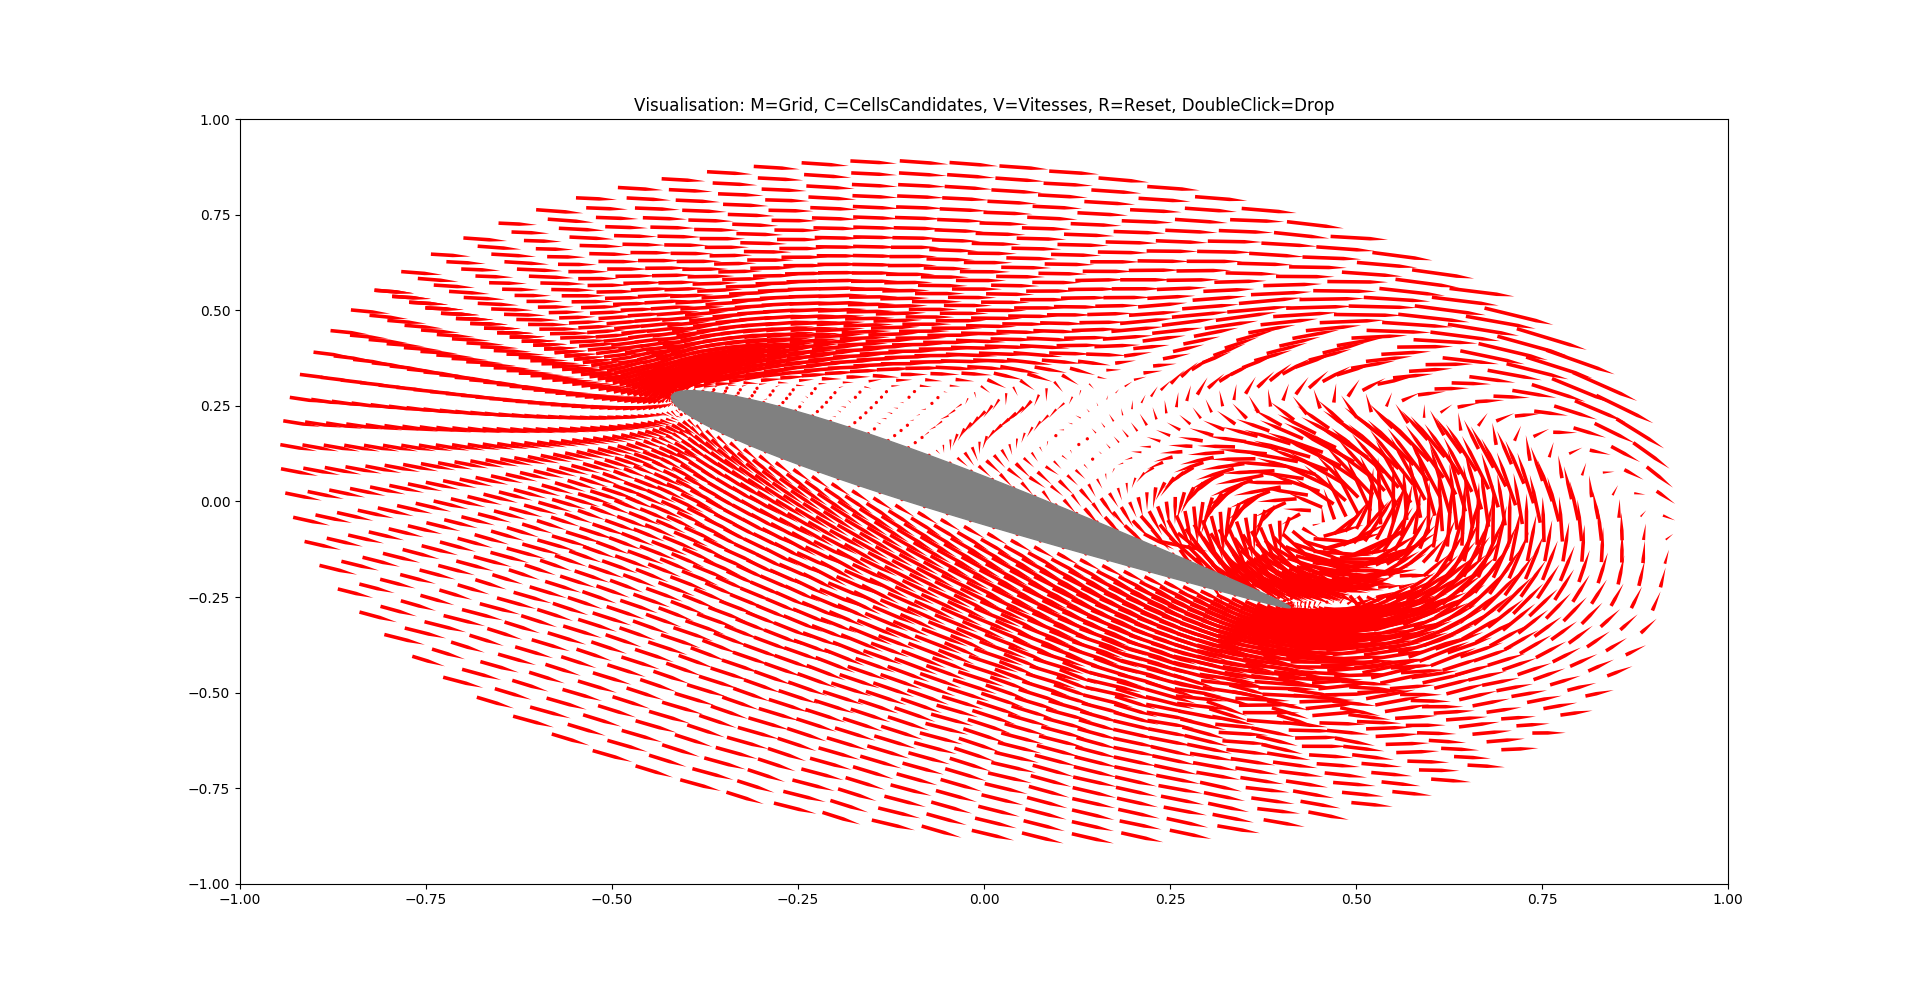
\includegraphics{docs/matplotlib_v.png}

   \begin{Verbatim}[commandchars=\\\{\},fontsize=\scriptsize]
{\color{incolor}In [{\color{incolor} }]:} \PY{c+c1}{\PYZsh{} Afficher le champs de vecteurs}
        \PY{k}{def} \PY{n+nf}{afficher\PYZus{}vitesse}\PY{p}{(}\PY{n+nb+bp}{self}\PY{p}{)}\PY{p}{:}
            \PY{n}{x}\PY{p}{,} \PY{n}{y}\PY{p}{,} \PY{n}{u}\PY{p}{,} \PY{n}{v} \PY{o}{=} \PY{n+nb+bp}{self}\PY{o}{.}\PY{n}{\PYZus{}\PYZus{}coords}\PY{p}{[}\PY{p}{:}\PY{p}{,} \PY{l+m+mi}{0}\PY{p}{]}\PY{p}{,} \PY{n+nb+bp}{self}\PY{o}{.}\PY{n}{\PYZus{}\PYZus{}coords}\PY{p}{[}\PY{p}{:}\PY{p}{,} \PY{l+m+mi}{1}\PY{p}{]}\PY{p}{,} \PY{n+nb+bp}{self}\PY{o}{.}\PY{n}{\PYZus{}\PYZus{}values}\PY{p}{[}\PY{p}{:}\PY{p}{,} \PY{l+m+mi}{0}\PY{p}{]}\PY{p}{,}
        \PY{n+nb+bp}{self}\PY{o}{.}\PY{n}{\PYZus{}\PYZus{}values}\PY{p}{[}\PY{p}{:}\PY{p}{,} \PY{l+m+mi}{1}\PY{p}{]}
            \PY{n}{ax}\PY{o}{.}\PY{n}{quiver}\PY{p}{(}\PY{n}{x}\PY{p}{,} \PY{n}{y}\PY{p}{,} \PY{n}{u}\PY{p}{,} \PY{n}{v}\PY{p}{,} \PY{n}{color}\PY{o}{=}\PY{l+s+s2}{\PYZdq{}}\PY{l+s+s2}{red}\PY{l+s+s2}{\PYZdq{}}\PY{p}{,} \PY{n}{headwidth}\PY{o}{=}\PY{l+m+mi}{1}\PY{p}{,} \PY{n}{scale}\PY{o}{=}\PY{l+m+mi}{35}\PY{p}{)}
\end{Verbatim}

    \hypertarget{fonction-pour-afficher-le-profil}{%
\subsection{Fonction pour afficher le
profil}\label{fonction-pour-afficher-le-profil}}

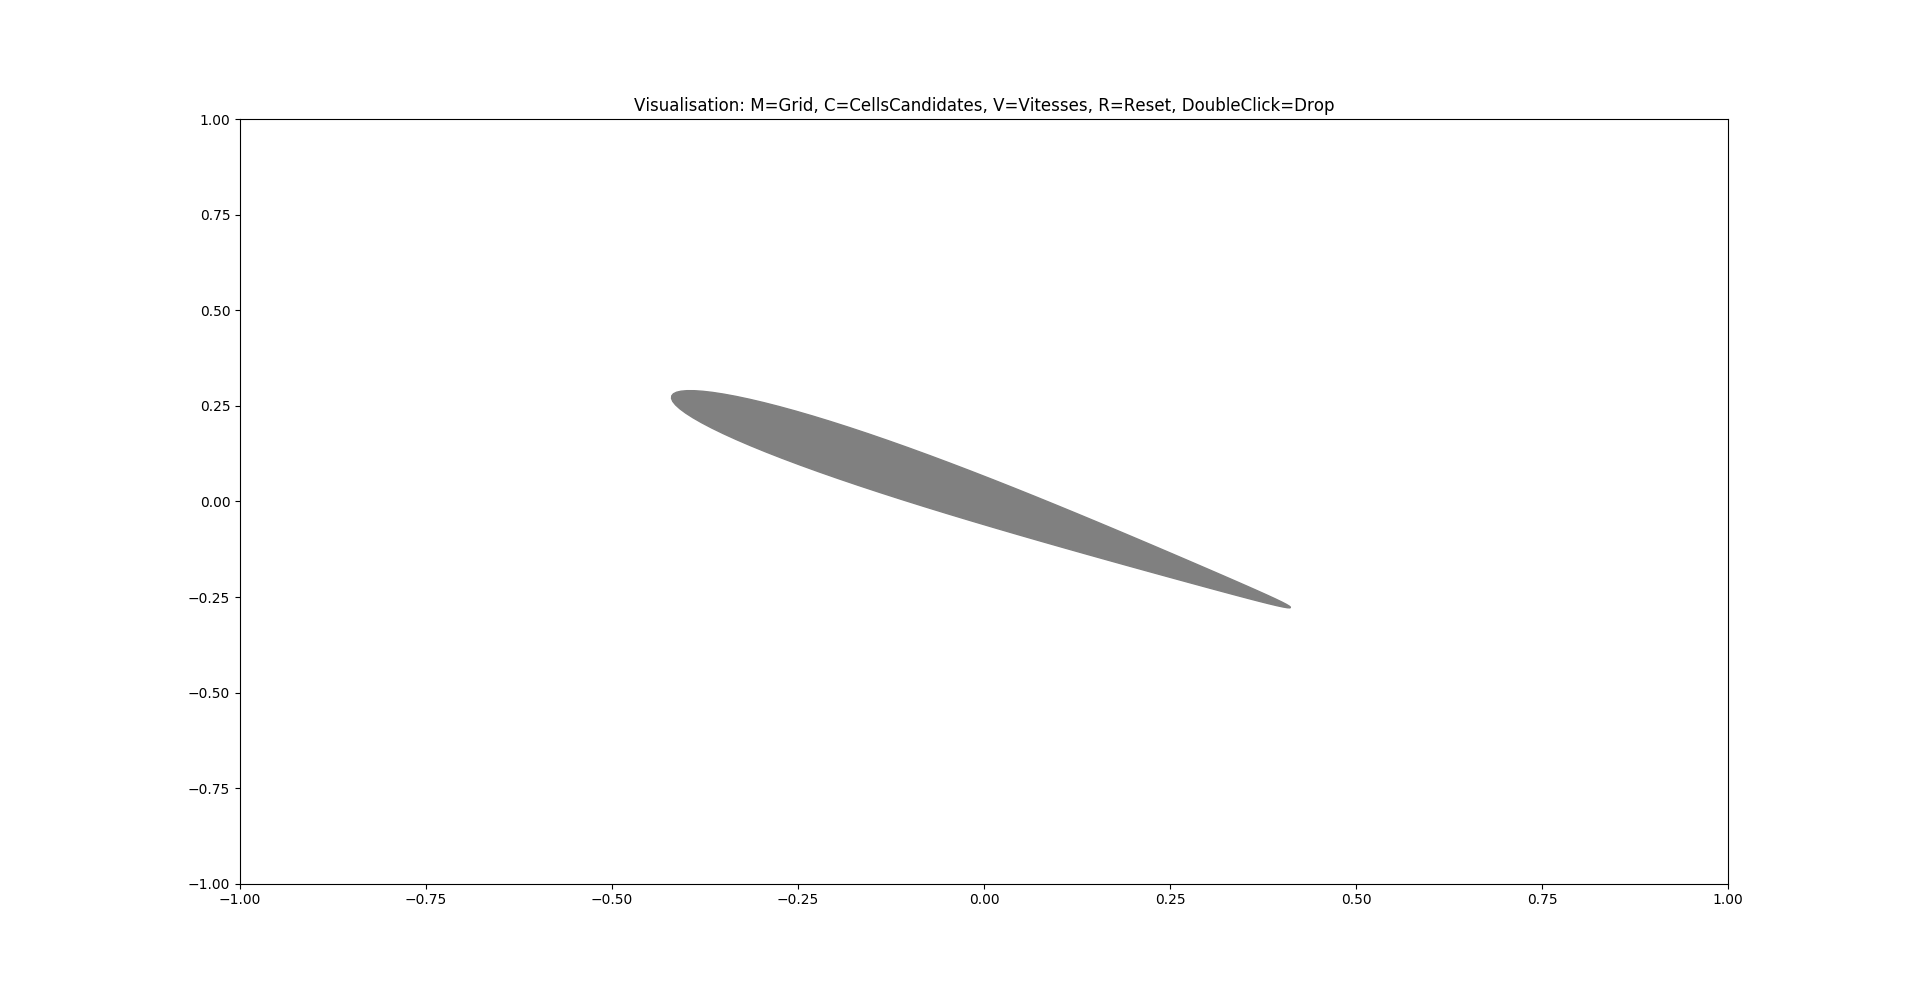
\includegraphics{docs/matplotlib_p.png}

   \begin{Verbatim}[commandchars=\\\{\},fontsize=\scriptsize]
{\color{incolor}In [{\color{incolor} }]:} \PY{c+c1}{\PYZsh{} Afficher le profil}
        \PY{k}{def} \PY{n+nf}{afficher\PYZus{}profil}\PY{p}{(}\PY{n+nb+bp}{self}\PY{p}{,} \PY{n}{color}\PY{p}{)}\PY{p}{:}
            \PY{n}{verts} \PY{o}{=} \PY{n+nb+bp}{self}\PY{o}{.}\PY{n}{\PYZus{}\PYZus{}coords}\PY{p}{[}\PY{l+m+mi}{0}\PY{p}{:}\PY{n+nb}{len}\PY{p}{(}\PY{n+nb+bp}{self}\PY{o}{.}\PY{n}{\PYZus{}\PYZus{}coords}\PY{p}{)}\PY{p}{:}\PY{l+m+mi}{35}\PY{p}{]}
            \PY{n}{poly} \PY{o}{=} \PY{n}{Polygon}\PY{p}{(}\PY{n}{verts}\PY{p}{)}
            \PY{n}{poly}\PY{o}{.}\PY{n}{set\PYZus{}color}\PY{p}{(}\PY{n}{color}\PY{p}{)}
            \PY{n}{ax}\PY{o}{.}\PY{n}{add\PYZus{}patch}\PY{p}{(}\PY{n}{poly}\PY{p}{)}
\end{Verbatim}

    \hypertarget{fonction-pour-afficher-le-maillage}{%
\subsection{Fonction pour afficher le
maillage}\label{fonction-pour-afficher-le-maillage}}

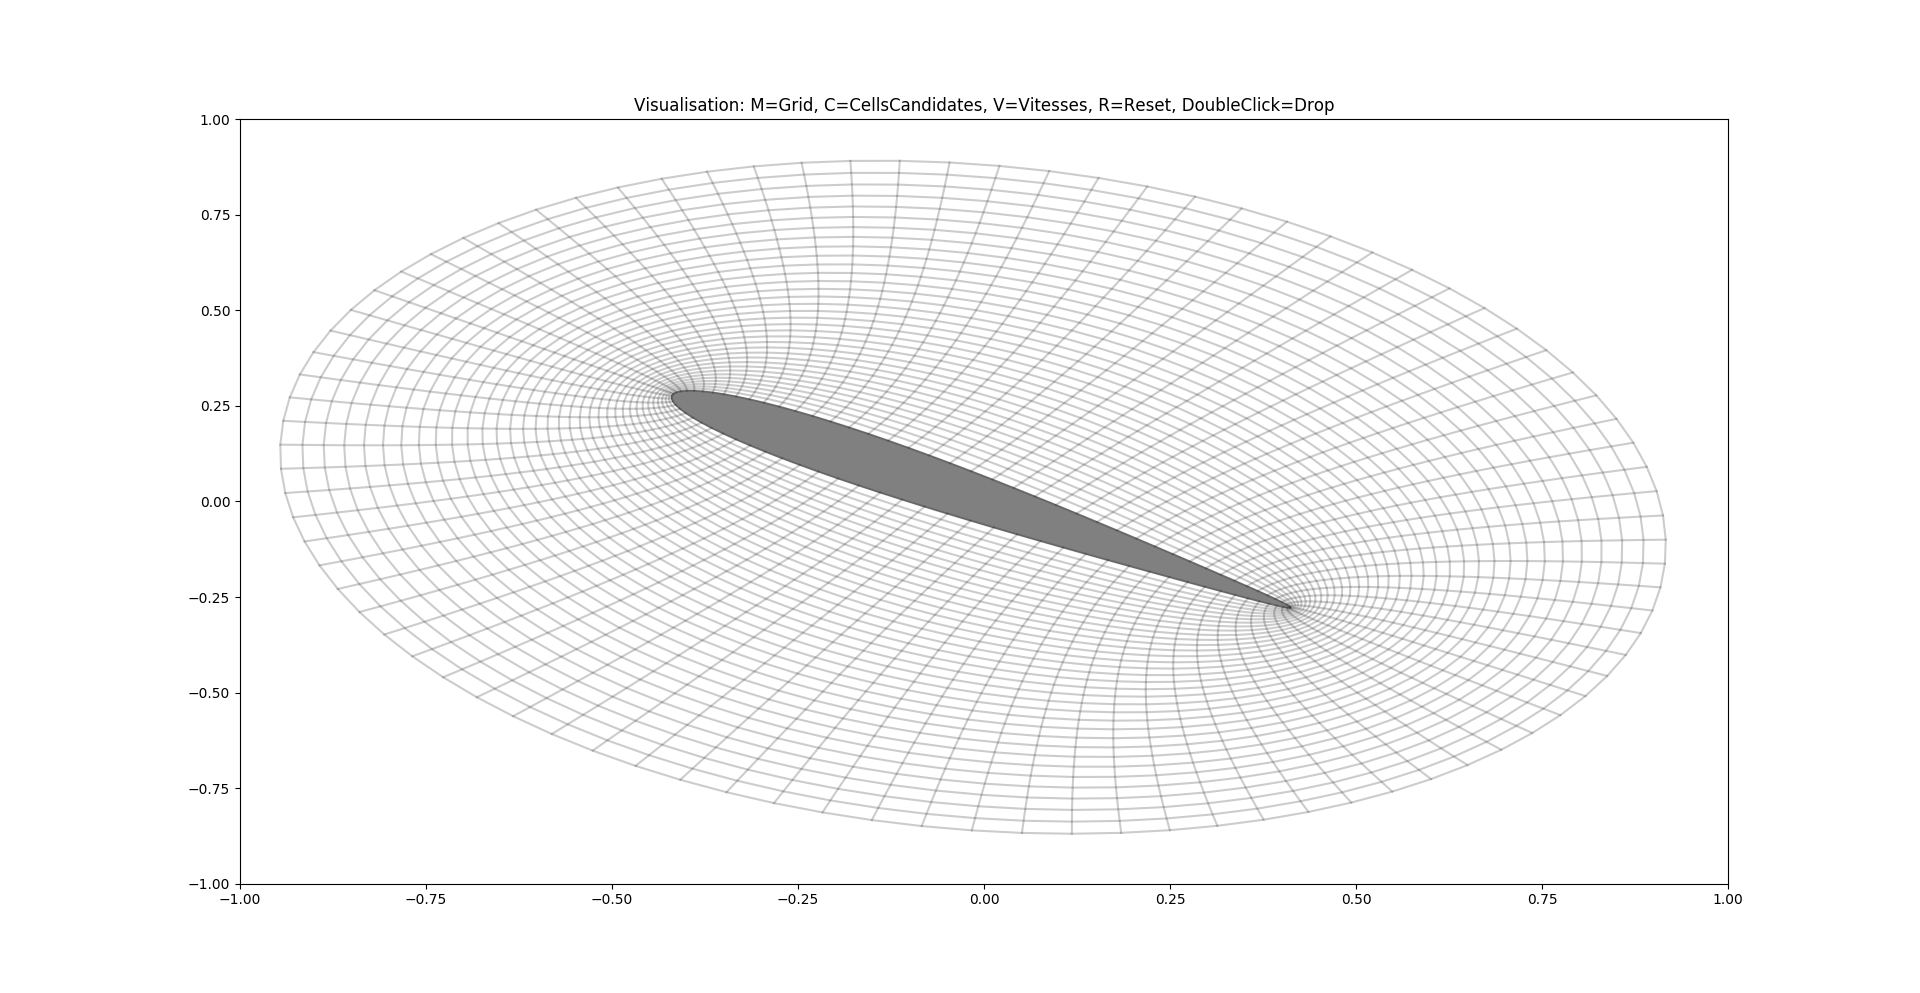
\includegraphics{docs/matplotlib_m.png}

   \begin{Verbatim}[commandchars=\\\{\},fontsize=\scriptsize]
{\color{incolor}In [{\color{incolor} }]:} \PY{c+c1}{\PYZsh{} Afficher le maillage}
        \PY{k}{def} \PY{n+nf}{afficher\PYZus{}maillage}\PY{p}{(}\PY{n+nb+bp}{self}\PY{p}{)}\PY{p}{:}
            \PY{n}{tabX}\PY{p}{,} \PY{n}{tabY} \PY{o}{=} \PY{n}{np}\PY{o}{.}\PY{n}{array}\PY{p}{(}\PY{n+nb+bp}{self}\PY{o}{.}\PY{n}{\PYZus{}\PYZus{}coords}\PY{p}{[}\PY{p}{:}\PY{p}{,} \PY{l+m+mi}{0}\PY{p}{]}\PY{p}{)}\PY{p}{,} \PY{n}{np}\PY{o}{.}\PY{n}{array}\PY{p}{(}\PY{n+nb+bp}{self}\PY{o}{.}\PY{n}{\PYZus{}\PYZus{}coords}\PY{p}{[}\PY{p}{:}\PY{p}{,} \PY{l+m+mi}{1}\PY{p}{]}\PY{p}{)}
        
            \PY{c+c1}{\PYZsh{} Vertical lines}
            \PY{k}{for} \PY{n}{n} \PY{o+ow}{in} \PY{n+nb}{range}\PY{p}{(}\PY{l+m+mi}{0}\PY{p}{,} \PY{l+m+mi}{35} \PY{o}{*} \PY{l+m+mi}{87}\PY{p}{,} \PY{l+m+mi}{35}\PY{p}{)}\PY{p}{:}
                \PY{n}{xs}\PY{p}{,} \PY{n}{ys} \PY{o}{=} \PY{n}{tabX}\PY{p}{[}\PY{n}{n}\PY{p}{:}\PY{n}{n} \PY{o}{+} \PY{l+m+mi}{35}\PY{p}{]}\PY{p}{,} \PY{n}{tabY}\PY{p}{[}\PY{n}{n}\PY{p}{:}\PY{n}{n} \PY{o}{+} \PY{l+m+mi}{35}\PY{p}{]}
                \PY{n}{plt}\PY{o}{.}\PY{n}{plot}\PY{p}{(}\PY{n}{xs}\PY{p}{,} \PY{n}{ys}\PY{p}{,} \PY{n}{c}\PY{o}{=}\PY{p}{(}\PY{l+m+mi}{0}\PY{p}{,} \PY{l+m+mi}{0}\PY{p}{,} \PY{l+m+mi}{0}\PY{p}{,} \PY{o}{.}\PY{l+m+mi}{2}\PY{p}{)}\PY{p}{)}
        
            \PY{c+c1}{\PYZsh{} Horizontal lines}
            \PY{k}{for} \PY{n}{n} \PY{o+ow}{in} \PY{n+nb}{range}\PY{p}{(}\PY{l+m+mi}{0}\PY{p}{,} \PY{l+m+mi}{35}\PY{p}{)}\PY{p}{:}
                \PY{n}{xs}\PY{p}{,} \PY{n}{ys} \PY{o}{=} \PY{n}{tabX}\PY{p}{[}\PY{n}{n}\PY{p}{:}\PY{n+nb}{len}\PY{p}{(}\PY{n}{tabX}\PY{p}{)}\PY{p}{:}\PY{l+m+mi}{35}\PY{p}{]}\PY{p}{,} \PY{n}{tabY}\PY{p}{[}\PY{n}{n}\PY{p}{:}\PY{n+nb}{len}\PY{p}{(}\PY{n}{tabY}\PY{p}{)}\PY{p}{:}\PY{l+m+mi}{35}\PY{p}{]}
                \PY{n}{plt}\PY{o}{.}\PY{n}{plot}\PY{p}{(}\PY{n}{xs}\PY{p}{,} \PY{n}{ys}\PY{p}{,} \PY{n}{c}\PY{o}{=}\PY{p}{(}\PY{l+m+mi}{0}\PY{p}{,} \PY{l+m+mi}{0}\PY{p}{,} \PY{l+m+mi}{0}\PY{p}{,} \PY{o}{.}\PY{l+m+mi}{2}\PY{p}{)}\PY{p}{)}
\end{Verbatim}

    \hypertarget{fonction-pour-affcicher-les-cellules-candidates}{%
\subsection{Fonction pour affcicher les cellules
candidates}\label{fonction-pour-affcicher-les-cellules-candidates}}

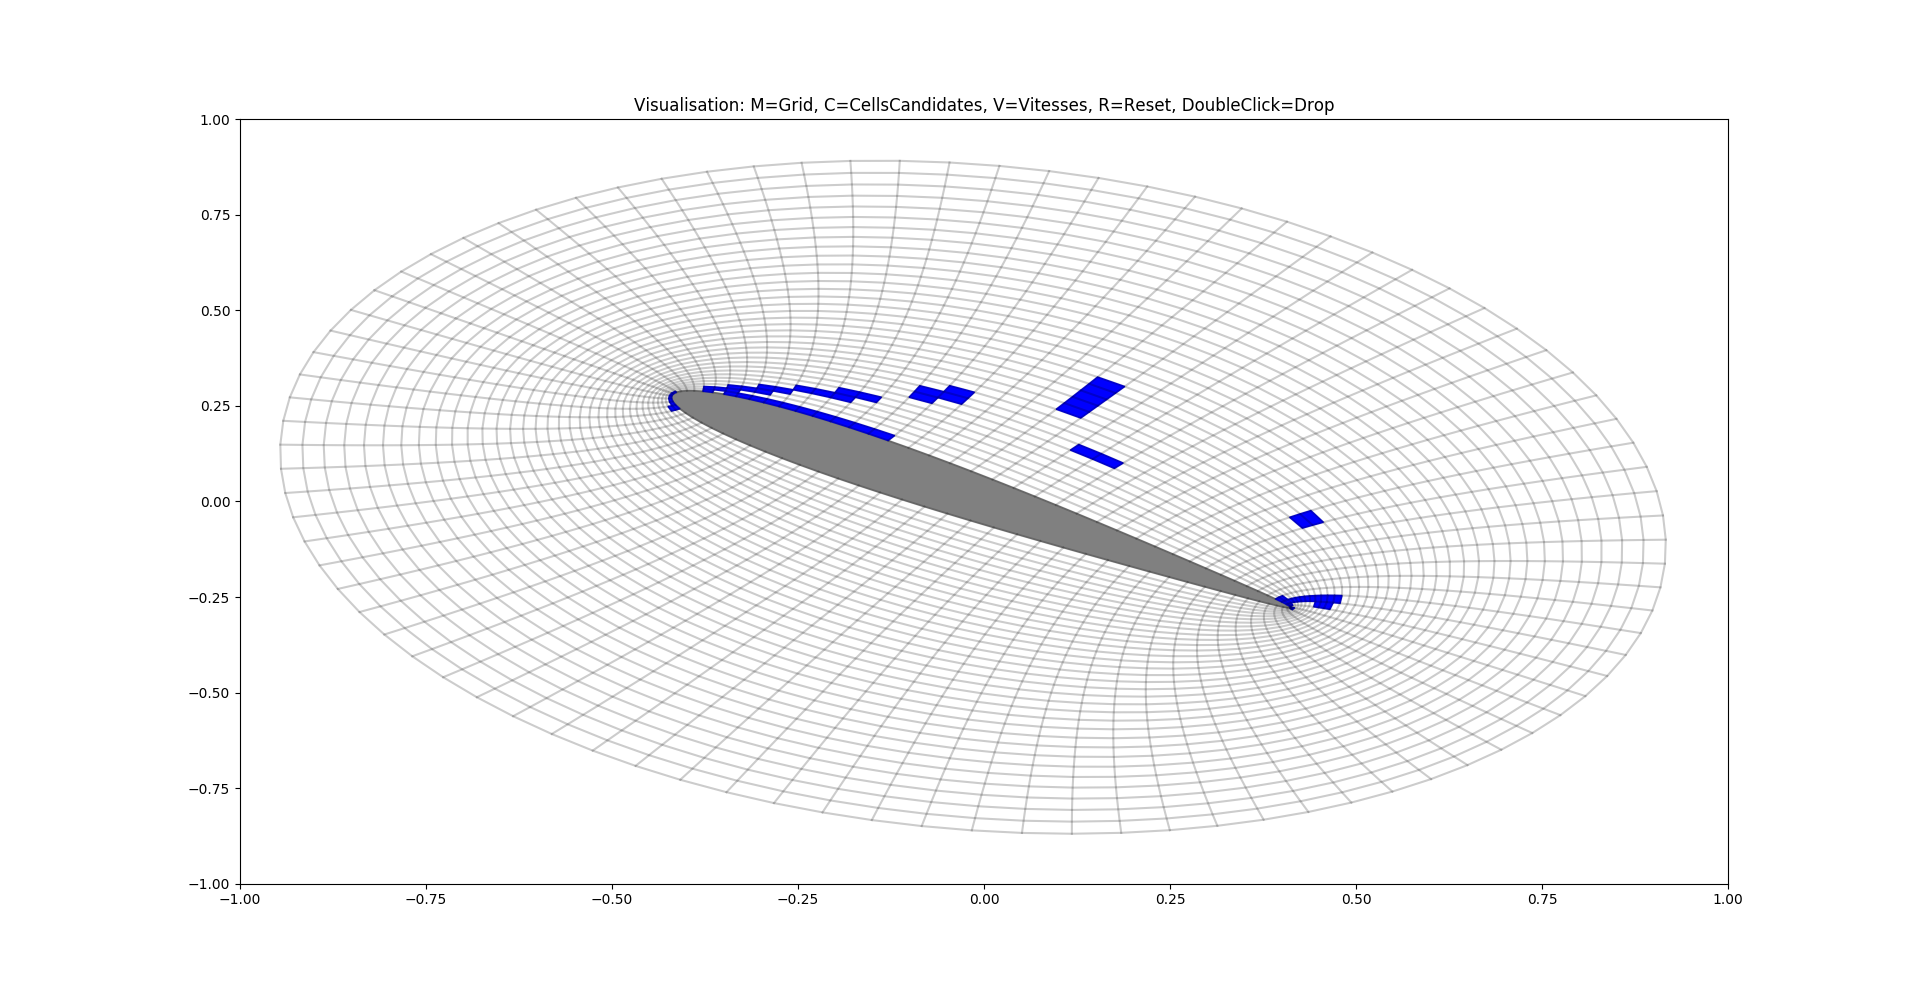
\includegraphics{docs/matplotlib_c.png}

   \begin{Verbatim}[commandchars=\\\{\},fontsize=\scriptsize]
{\color{incolor}In [{\color{incolor} }]:} \PY{c+c1}{\PYZsh{} Afficher les cellules candidates:}
        \PY{k}{def} \PY{n+nf}{afficher\PYZus{}cellules}\PY{p}{(}\PY{n+nb+bp}{self}\PY{p}{,} \PY{n}{color}\PY{p}{)}\PY{p}{:}
        
            \PY{c+c1}{\PYZsh{} test sign}
            \PY{k}{def} \PY{n+nf}{test\PYZus{}sign}\PY{p}{(}\PY{n}{vectors}\PY{p}{)}\PY{p}{:}
                \PY{k}{for} \PY{n}{i} \PY{o+ow}{in} \PY{n+nb}{range}\PY{p}{(}\PY{n+nb}{len}\PY{p}{(}\PY{n}{vectors}\PY{p}{)}\PY{o}{\PYZhy{}}\PY{l+m+mi}{1}\PY{p}{)}\PY{p}{:}
                    \PY{n}{vec1}\PY{p}{,} \PY{n}{vec2} \PY{o}{=} \PY{n}{vectors}\PY{p}{[}\PY{n}{i}\PY{p}{]}\PY{p}{,} \PY{n}{vectors}\PY{p}{[}\PY{n}{i}\PY{o}{+}\PY{l+m+mi}{1}\PY{p}{]}
        
                    \PY{c+c1}{\PYZsh{} Si le produit scalaire est négatif, alors les vecteurs sont opposés}
                    \PY{k}{if} \PY{n}{np}\PY{o}{.}\PY{n}{dot}\PY{p}{(}\PY{n}{vec1}\PY{p}{,} \PY{n}{vec2}\PY{p}{)} \PY{o}{\PYZlt{}} \PY{l+m+mi}{0}\PY{p}{:}
                        \PY{k}{return} \PY{k+kc}{False}
        
                \PY{k}{return} \PY{k+kc}{True}
        
            \PY{c+c1}{\PYZsh{} Begin}
            \PY{k}{for} \PY{n}{cell} \PY{o+ow}{in} \PY{n+nb+bp}{self}\PY{o}{.}\PY{n}{\PYZus{}\PYZus{}cells}\PY{p}{:}
                \PY{n}{x1}\PY{p}{,} \PY{n}{x2}\PY{p}{,} \PY{n}{x3}\PY{p}{,} \PY{n}{x4} \PY{o}{=} \PY{n}{cell}\PY{p}{[}\PY{p}{:}\PY{p}{,} \PY{l+m+mi}{0}\PY{p}{]}
                \PY{n}{y1}\PY{p}{,} \PY{n}{y2}\PY{p}{,} \PY{n}{y3}\PY{p}{,} \PY{n}{y4} \PY{o}{=} \PY{n}{cell}\PY{p}{[}\PY{p}{:}\PY{p}{,} \PY{l+m+mi}{1}\PY{p}{]}
                \PY{n}{u1}\PY{p}{,} \PY{n}{u2}\PY{p}{,} \PY{n}{u3}\PY{p}{,} \PY{n}{u4} \PY{o}{=} \PY{n}{cell}\PY{p}{[}\PY{p}{:}\PY{p}{,} \PY{l+m+mi}{2}\PY{p}{]}
                \PY{n}{v1}\PY{p}{,} \PY{n}{v2}\PY{p}{,} \PY{n}{v3}\PY{p}{,} \PY{n}{v4} \PY{o}{=} \PY{n}{cell}\PY{p}{[}\PY{p}{:}\PY{p}{,} \PY{l+m+mi}{3}\PY{p}{]}
        
                \PY{c+c1}{\PYZsh{} Les 4 vecteurs}
                \PY{n}{vecs} \PY{o}{=} \PY{p}{[} \PY{p}{[}\PY{n}{u1}\PY{p}{,} \PY{n}{v1}\PY{p}{]}\PY{p}{,} \PY{p}{[}\PY{n}{u2}\PY{p}{,} \PY{n}{v2}\PY{p}{]}\PY{p}{,} \PY{p}{[}\PY{n}{u3}\PY{p}{,} \PY{n}{v3}\PY{p}{]}\PY{p}{,} \PY{p}{[}\PY{n}{u4}\PY{p}{,} \PY{n}{v4}\PY{p}{]} \PY{p}{]}
        
                \PY{k}{if} \PY{o+ow}{not} \PY{n}{test\PYZus{}sign}\PY{p}{(}\PY{n}{vecs}\PY{p}{)}\PY{p}{:}
                    \PY{n}{verts} \PY{o}{=} \PY{p}{[} \PY{p}{(}\PY{n}{x1}\PY{p}{,} \PY{n}{y1}\PY{p}{)}\PY{p}{,} \PY{p}{(}\PY{n}{x2}\PY{p}{,} \PY{n}{y2}\PY{p}{)}\PY{p}{,} \PY{p}{(}\PY{n}{x3}\PY{p}{,} \PY{n}{y3}\PY{p}{)}\PY{p}{,} \PY{p}{(}\PY{n}{x4}\PY{p}{,} \PY{n}{y4}\PY{p}{)} \PY{p}{]}
                    \PY{n}{poly} \PY{o}{=} \PY{n}{Polygon}\PY{p}{(}\PY{n}{verts}\PY{p}{)}
                    \PY{n}{poly}\PY{o}{.}\PY{n}{set\PYZus{}color}\PY{p}{(}\PY{n}{color}\PY{p}{)}
                    \PY{n}{ax}\PY{o}{.}\PY{n}{add\PYZus{}patch}\PY{p}{(}\PY{n}{poly}\PY{p}{)}
\end{Verbatim}

    \hypertarget{fonction-pour-charger-les-objets}{%
\subsection{Fonction pour charger les
objets}\label{fonction-pour-charger-les-objets}}

   \begin{Verbatim}[commandchars=\\\{\},fontsize=\scriptsize]
{\color{incolor}In [{\color{incolor} }]:} \PY{k}{def} \PY{n+nf}{charger\PYZus{}objet}\PY{p}{(}\PY{n}{obj}\PY{p}{,} \PY{n}{limit}\PY{o}{=}\PY{l+m+mi}{0}\PY{p}{)}\PY{p}{:}
            \PY{n}{coords} \PY{o}{=} \PY{p}{[}\PY{p}{]}
            \PY{n}{values} \PY{o}{=} \PY{p}{[}\PY{p}{]}
            \PY{n}{count} \PY{o}{=} \PY{l+m+mi}{0}
        
            \PY{n}{file} \PY{o}{=} \PY{n+nb}{open}\PY{p}{(}\PY{n}{obj}\PY{p}{,} \PY{l+s+s2}{\PYZdq{}}\PY{l+s+s2}{r}\PY{l+s+s2}{\PYZdq{}}\PY{p}{)}
            \PY{n}{angle} \PY{o}{=} \PY{l+m+mf}{0.}
            \PY{n}{x}\PY{p}{,} \PY{n}{y} \PY{o}{=} \PY{l+m+mf}{0.}\PY{p}{,} \PY{l+m+mf}{0.}
            \PY{n}{u}\PY{p}{,} \PY{n}{v} \PY{o}{=} \PY{l+m+mf}{0.}\PY{p}{,} \PY{l+m+mf}{0.}
        
            \PY{n}{R} \PY{o}{=} \PY{n}{np}\PY{o}{.}\PY{n}{zeros}\PY{p}{(}\PY{p}{(}\PY{l+m+mi}{2}\PY{p}{,} \PY{l+m+mi}{2}\PY{p}{)}\PY{p}{)}
        
            \PY{k}{for} \PY{n}{line} \PY{o+ow}{in} \PY{n}{file}\PY{o}{.}\PY{n}{readlines}\PY{p}{(}\PY{p}{)}\PY{p}{:}
                \PY{n}{data} \PY{o}{=} \PY{n}{line}\PY{o}{.}\PY{n}{split}\PY{p}{(}\PY{p}{)}
        
                \PY{k}{if} \PY{n}{count} \PY{o}{==} \PY{l+m+mi}{0}\PY{p}{:}
                    \PY{n}{angle} \PY{o}{=} \PY{n+nb}{float}\PY{p}{(}\PY{n}{data}\PY{p}{[}\PY{l+m+mi}{2}\PY{p}{]}\PY{p}{)}
        
                    \PY{n}{theta} \PY{o}{=} \PY{n}{np}\PY{o}{.}\PY{n}{radians}\PY{p}{(}\PY{n}{angle}\PY{p}{)}
                    \PY{n}{c}\PY{p}{,} \PY{n}{s} \PY{o}{=} \PY{n}{np}\PY{o}{.}\PY{n}{cos}\PY{p}{(}\PY{n}{theta}\PY{p}{)}\PY{p}{,} \PY{n}{np}\PY{o}{.}\PY{n}{sin}\PY{p}{(}\PY{n}{theta}\PY{p}{)}
                    \PY{n}{R} \PY{o}{=} \PY{n}{np}\PY{o}{.}\PY{n}{array}\PY{p}{(}\PY{p}{(}\PY{p}{(}\PY{n}{c}\PY{p}{,} \PY{o}{\PYZhy{}}\PY{n}{s}\PY{p}{)}\PY{p}{,} \PY{p}{(}\PY{n}{s}\PY{p}{,} \PY{n}{c}\PY{p}{)}\PY{p}{)}\PY{p}{)}
        
                    \PY{n}{count} \PY{o}{+}\PY{o}{=} \PY{l+m+mi}{1}
                    \PY{k}{continue}
        
                \PY{n}{x}\PY{p}{,} \PY{n}{y}\PY{p}{,} \PY{n}{u}\PY{p}{,} \PY{n}{v} \PY{o}{=} \PY{n+nb}{float}\PY{p}{(}\PY{n}{data}\PY{p}{[}\PY{l+m+mi}{0}\PY{p}{]}\PY{p}{)}\PY{p}{,} \PY{n+nb}{float}\PY{p}{(}\PY{n}{data}\PY{p}{[}\PY{l+m+mi}{1}\PY{p}{]}\PY{p}{)}\PY{p}{,} \PY{n+nb}{float}\PY{p}{(}\PY{n}{data}\PY{p}{[}\PY{l+m+mi}{2}\PY{p}{]}\PY{p}{)}\PY{p}{,} \PY{n+nb}{float}\PY{p}{(}\PY{n}{data}\PY{p}{[}\PY{l+m+mi}{3}\PY{p}{]}\PY{p}{)}
        
                \PY{c+c1}{\PYZsh{} Rotation matrix}
                \PY{n}{coords}\PY{o}{.}\PY{n}{append}\PY{p}{(}\PY{n}{np}\PY{o}{.}\PY{n}{matmul}\PY{p}{(}\PY{n}{R}\PY{p}{,} \PY{n}{np}\PY{o}{.}\PY{n}{array}\PY{p}{(}\PY{p}{(}\PY{n}{x}\PY{p}{,} \PY{n}{y}\PY{p}{)}\PY{p}{)}\PY{p}{)}\PY{p}{)}
                \PY{n}{values}\PY{o}{.}\PY{n}{append}\PY{p}{(}\PY{n}{np}\PY{o}{.}\PY{n}{matmul}\PY{p}{(}\PY{n}{R}\PY{p}{,} \PY{n}{np}\PY{o}{.}\PY{n}{array}\PY{p}{(}\PY{p}{(}\PY{n}{u}\PY{p}{,} \PY{n}{v}\PY{p}{)}\PY{p}{)}\PY{p}{)}\PY{p}{)}
        
                \PY{k}{if} \PY{n}{limit} \PY{o}{!=} \PY{l+m+mi}{0} \PY{o+ow}{and} \PY{n}{count} \PY{o}{==} \PY{n}{limit}\PY{p}{:} \PY{k}{break}
                \PY{n}{count} \PY{o}{+}\PY{o}{=} \PY{l+m+mi}{1}
        
            \PY{k}{return} \PY{n}{np}\PY{o}{.}\PY{n}{array}\PY{p}{(}\PY{n}{coords}\PY{p}{)}\PY{p}{,} \PY{n}{np}\PY{o}{.}\PY{n}{array}\PY{p}{(}\PY{n}{values}\PY{p}{)}
\end{Verbatim}

    \hypertarget{fonction-pour-afficher-les-objets}{%
\subsection{Fonction pour afficher les
objets}\label{fonction-pour-afficher-les-objets}}

   \begin{Verbatim}[commandchars=\\\{\},fontsize=\scriptsize]
{\color{incolor}In [{\color{incolor} }]:} \PY{c+c1}{\PYZsh{} Afficher l\PYZsq{}objet}
        \PY{k}{def} \PY{n+nf}{afficher\PYZus{}objet}\PY{p}{(}\PY{n+nb+bp}{self}\PY{p}{)}\PY{p}{:}
        
            \PY{n}{plt}\PY{o}{.}\PY{n}{cla}\PY{p}{(}\PY{p}{)}
        
            \PY{n+nb+bp}{self}\PY{o}{.}\PY{n}{afficher\PYZus{}profil}\PY{p}{(}\PY{l+s+s2}{\PYZdq{}}\PY{l+s+s2}{grey}\PY{l+s+s2}{\PYZdq{}}\PY{p}{)}
            \PY{k}{if} \PY{n+nb+bp}{self}\PY{o}{.}\PY{n}{\PYZus{}\PYZus{}dispVec}\PY{p}{:}
                \PY{n+nb+bp}{self}\PY{o}{.}\PY{n}{afficher\PYZus{}vitesse}\PY{p}{(}\PY{p}{)}
            \PY{k}{if} \PY{n+nb+bp}{self}\PY{o}{.}\PY{n}{\PYZus{}\PYZus{}dispGrid}\PY{p}{:}
                \PY{n+nb+bp}{self}\PY{o}{.}\PY{n}{afficher\PYZus{}maillage}\PY{p}{(}\PY{p}{)}
            \PY{k}{if} \PY{n+nb+bp}{self}\PY{o}{.}\PY{n}{\PYZus{}\PYZus{}dispCellule}\PY{p}{:}
                \PY{n+nb+bp}{self}\PY{o}{.}\PY{n}{afficher\PYZus{}cellules}\PY{p}{(}\PY{l+s+s2}{\PYZdq{}}\PY{l+s+s2}{blue}\PY{l+s+s2}{\PYZdq{}}\PY{p}{)}
        
            \PY{c+c1}{\PYZsh{}print([min(self.\PYZus{}\PYZus{}coords[:, 0]), max(self.\PYZus{}\PYZus{}coords[:, 0]), min(self.\PYZus{}\PYZus{}coords[:,}
        \PY{l+m+mi}{1}\PY{p}{]}\PY{p}{)}\PY{p}{,} \PY{n+nb}{max}\PY{p}{(}\PY{n+nb+bp}{self}\PY{o}{.}\PY{n}{\PYZus{}\PYZus{}coords}\PY{p}{[}\PY{p}{:}\PY{p}{,} \PY{l+m+mi}{1}\PY{p}{]}\PY{p}{)}\PY{p}{]}\PY{p}{)}
            \PY{n}{ax}\PY{o}{.}\PY{n}{set\PYZus{}xlim}\PY{p}{(}\PY{o}{\PYZhy{}}\PY{l+m+mi}{1}\PY{p}{,} \PY{l+m+mi}{1}\PY{p}{)}
            \PY{n}{ax}\PY{o}{.}\PY{n}{set\PYZus{}ylim}\PY{p}{(}\PY{o}{\PYZhy{}}\PY{l+m+mi}{1}\PY{p}{,} \PY{l+m+mi}{1}\PY{p}{)}
        
            \PY{c+c1}{\PYZsh{} draw lines}
            \PY{n+nb+bp}{self}\PY{o}{.}\PY{n}{calcul\PYZus{}lignes}\PY{p}{(}\PY{p}{)}
        
            \PY{n}{plt}\PY{o}{.}\PY{n}{title}\PY{p}{(}\PY{l+s+s1}{\PYZsq{}}\PY{l+s+s1}{Visualisation: M=Grid, C=CellsCandidates, V=Vitesses, R=Reset,}
        \PY{n}{DoubleClick}\PY{o}{=}\PY{n}{Drop}\PY{l+s+s1}{\PYZsq{}}\PY{l+s+s1}{)}
            \PY{n}{plt}\PY{o}{.}\PY{n}{show}\PY{p}{(}\PY{p}{)}
\end{Verbatim}

    \hypertarget{fonction-pour-simuler-le-luxe2chage-des-particules-dans-le-champ-des-vitesses}{%
\subsection{Fonction pour simuler le lâchage des particules dans le
champ des
vitesses}\label{fonction-pour-simuler-le-luxe2chage-des-particules-dans-le-champ-des-vitesses}}

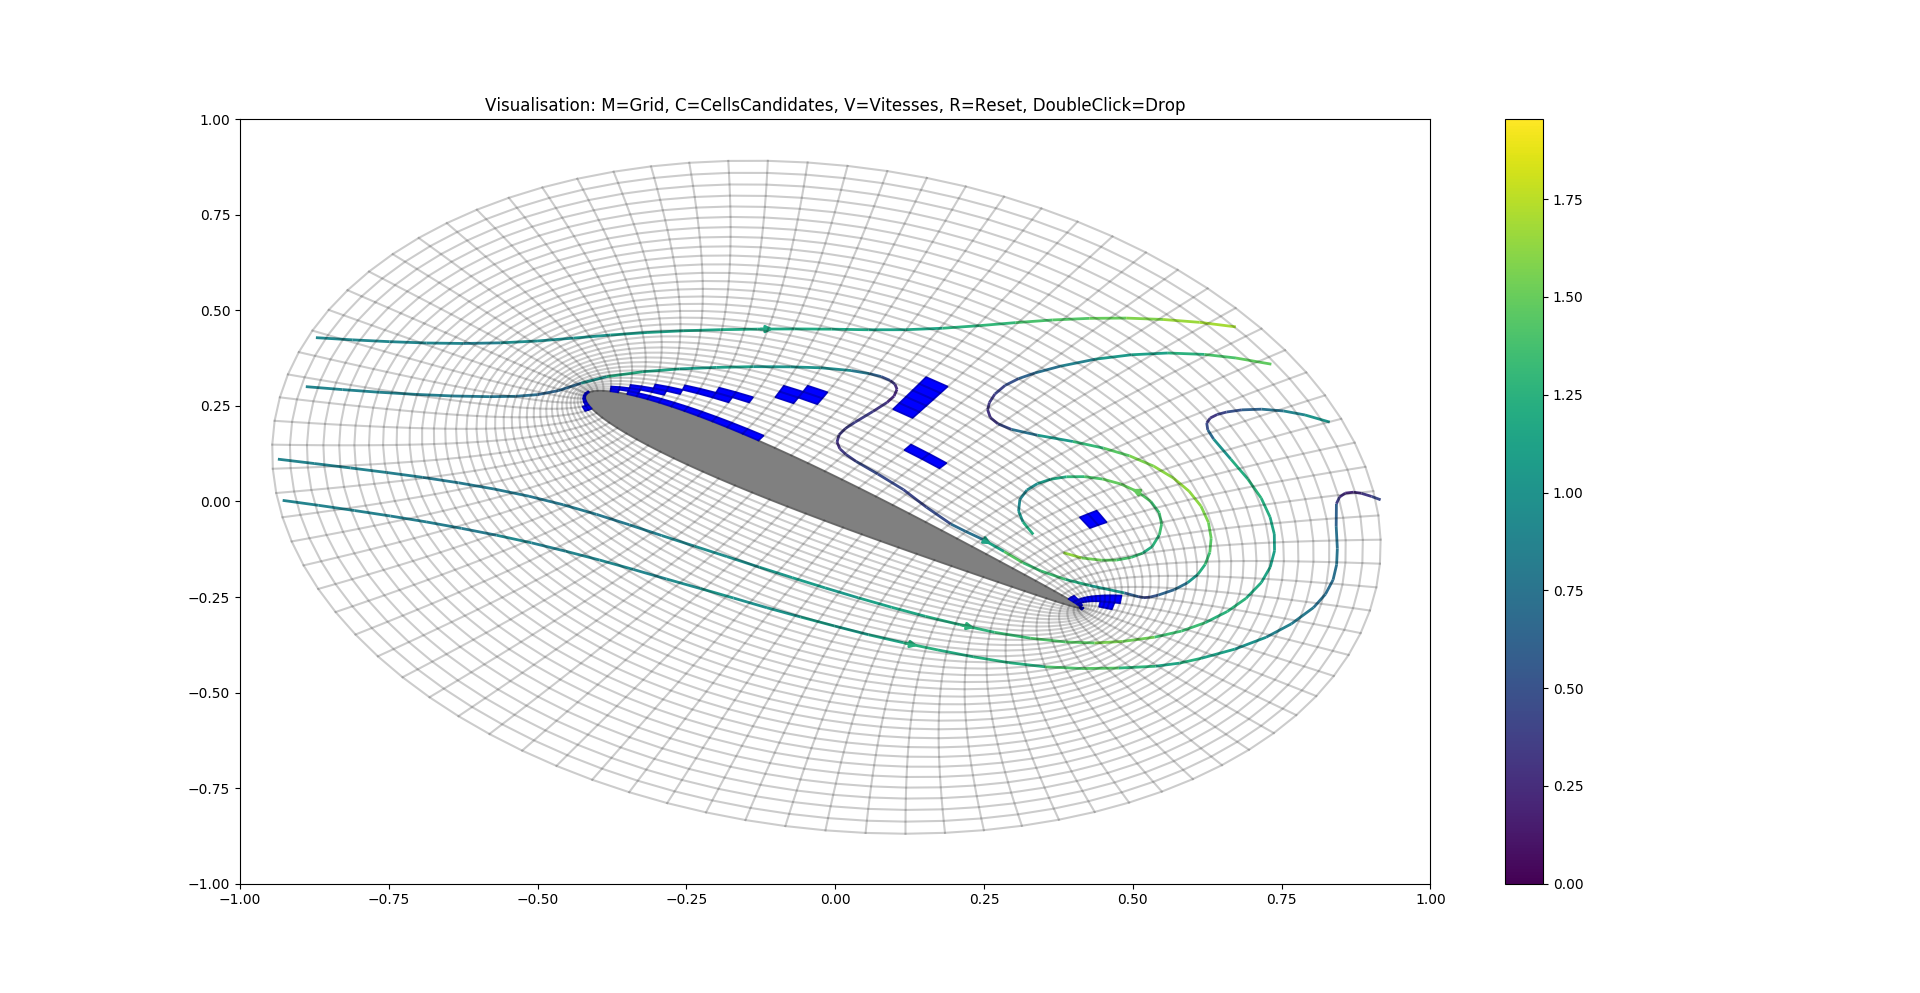
\includegraphics{docs/matplotlib_lines.png}

   \begin{Verbatim}[commandchars=\\\{\},fontsize=\scriptsize]
{\color{incolor}In [{\color{incolor} }]:} \PY{c+c1}{\PYZsh{} calcul\PYZus{}lignes}
        \PY{k}{def} \PY{n+nf}{calcul\PYZus{}lignes}\PY{p}{(}\PY{n+nb+bp}{self}\PY{p}{)}\PY{p}{:}
            \PY{k}{if}\PY{p}{(}\PY{n+nb}{len}\PY{p}{(}\PY{n+nb+bp}{self}\PY{o}{.}\PY{n}{\PYZus{}\PYZus{}dropPoints}\PY{p}{)} \PY{o}{\PYZgt{}} \PY{l+m+mi}{0}\PY{p}{)}\PY{p}{:}
                \PY{n}{strm} \PY{o}{=} \PY{n}{ax}\PY{o}{.}\PY{n}{streamplot}\PY{p}{(}\PY{n+nb+bp}{self}\PY{o}{.}\PY{n}{\PYZus{}\PYZus{}xs}\PY{p}{,} \PY{n+nb+bp}{self}\PY{o}{.}\PY{n}{\PYZus{}\PYZus{}ys}\PY{p}{,} \PY{n+nb+bp}{self}\PY{o}{.}\PY{n}{\PYZus{}\PYZus{}us}\PY{p}{,} \PY{n+nb+bp}{self}\PY{o}{.}\PY{n}{\PYZus{}\PYZus{}vs}\PY{p}{,}
        \PY{n}{start\PYZus{}points}\PY{o}{=}\PY{n+nb+bp}{self}\PY{o}{.}\PY{n}{\PYZus{}\PYZus{}dropPoints}\PY{p}{,} \PY{n}{color}\PY{o}{=}\PY{n+nb+bp}{self}\PY{o}{.}\PY{n}{\PYZus{}\PYZus{}speeds}\PY{p}{,} \PY{n}{linewidth}\PY{o}{=}\PY{l+m+mi}{2}\PY{p}{,} \PY{n}{cmap}\PY{o}{=}\PY{l+s+s2}{\PYZdq{}}\PY{l+s+s2}{viridis}\PY{l+s+s2}{\PYZdq{}}\PY{p}{)}
                \PY{k}{if} \PY{n+nb+bp}{self}\PY{o}{.}\PY{n}{\PYZus{}\PYZus{}strm} \PY{o+ow}{is} \PY{k+kc}{None}\PY{p}{:}
                    \PY{n+nb+bp}{self}\PY{o}{.}\PY{n}{\PYZus{}\PYZus{}strm} \PY{o}{=} \PY{n}{strm}
                    \PY{n+nb+bp}{self}\PY{o}{.}\PY{n}{\PYZus{}\PYZus{}colorbar} \PY{o}{=} \PY{n}{fig}\PY{o}{.}\PY{n}{colorbar}\PY{p}{(}\PY{n}{strm}\PY{o}{.}\PY{n}{lines}\PY{p}{)}
\end{Verbatim}

    \hypertarget{pyvtk}{%
\section{PyVTK}\label{pyvtk}}

Pour cette partie, nous allons utiliser
\href{https://github.com/vtkiorg/vtki}{VTKI}, une interface de VTK pour
Python. Elle offre les fonctionalités ressemblables à celles de
Matplotlib, avec une documentation assez élaborée.

Malgré tout, je n'ai pas eu le temps nécessaire pour adapter le code
fait avec Matplotlib à VTKi, on voit encore dans le fichier
\texttt{vtki\_viz.py}, les traces de ceux qui ont été réalisés.

Cependant, on peut voir un exemple de code qui permet de afficher un
champs de vecteurs:

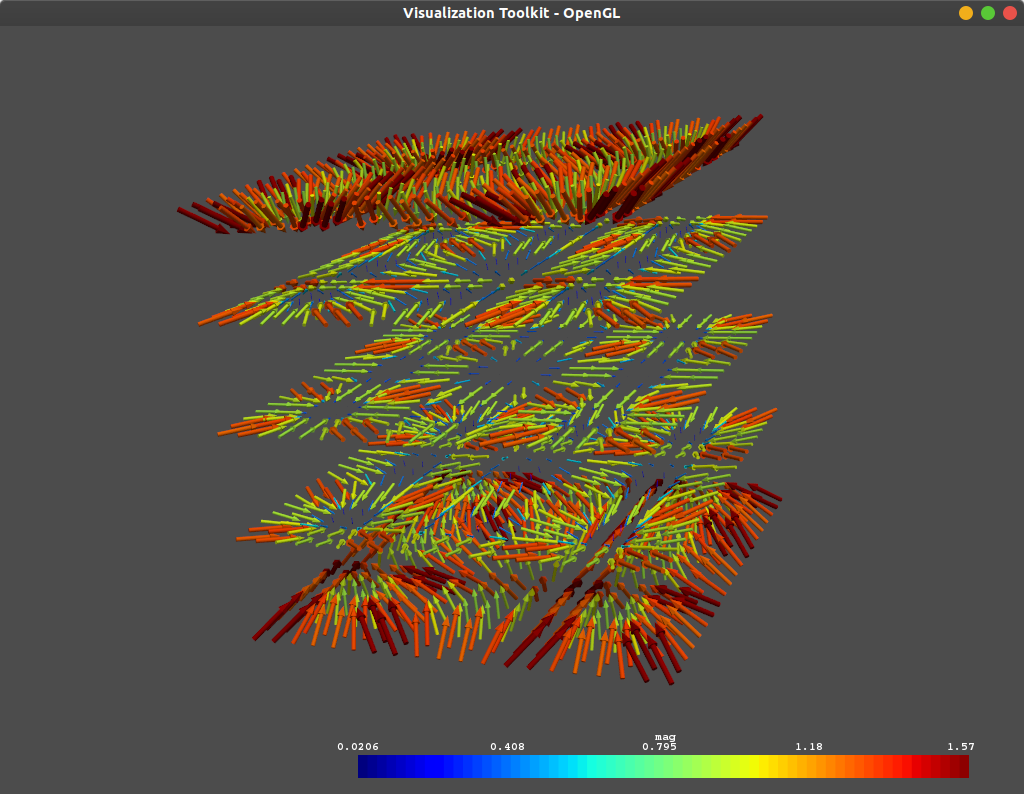
\includegraphics{docs/vtk_glyphes.png}

   \begin{Verbatim}[commandchars=\\\{\},fontsize=\scriptsize]
{\color{incolor}In [{\color{incolor} }]:} \PY{k+kn}{import} \PY{n+nn}{vtki}
        \PY{k+kn}{import} \PY{n+nn}{numpy} \PY{k}{as} \PY{n+nn}{np}
        
        \PY{c+c1}{\PYZsh{} Make a grid:}
        \PY{n}{x}\PY{p}{,} \PY{n}{y}\PY{p}{,} \PY{n}{z} \PY{o}{=} \PY{n}{np}\PY{o}{.}\PY{n}{meshgrid}\PY{p}{(}\PY{n}{np}\PY{o}{.}\PY{n}{linspace}\PY{p}{(}\PY{o}{\PYZhy{}}\PY{l+m+mi}{5}\PY{p}{,} \PY{l+m+mi}{5}\PY{p}{,} \PY{l+m+mi}{20}\PY{p}{)}\PY{p}{,}
                          \PY{n}{np}\PY{o}{.}\PY{n}{linspace}\PY{p}{(}\PY{o}{\PYZhy{}}\PY{l+m+mi}{5}\PY{p}{,} \PY{l+m+mi}{5}\PY{p}{,} \PY{l+m+mi}{20}\PY{p}{)}\PY{p}{,}
                          \PY{n}{np}\PY{o}{.}\PY{n}{linspace}\PY{p}{(}\PY{o}{\PYZhy{}}\PY{l+m+mi}{5}\PY{p}{,} \PY{l+m+mi}{5}\PY{p}{,} \PY{l+m+mi}{5}\PY{p}{)}\PY{p}{)}
        
        \PY{n}{grid} \PY{o}{=} \PY{n}{vtki}\PY{o}{.}\PY{n}{StructuredGrid}\PY{p}{(}\PY{n}{x}\PY{p}{,} \PY{n}{y}\PY{p}{,} \PY{n}{z}\PY{p}{)}
        
        \PY{n}{vectors} \PY{o}{=} \PY{n}{np}\PY{o}{.}\PY{n}{sin}\PY{p}{(}\PY{n}{grid}\PY{o}{.}\PY{n}{points}\PY{p}{)}\PY{o}{*}\PY{o}{*}\PY{l+m+mi}{3}
        
        
        \PY{c+c1}{\PYZsh{} Compute a direction for the vector field}
        \PY{n}{grid}\PY{o}{.}\PY{n}{point\PYZus{}arrays}\PY{p}{[}\PY{l+s+s1}{\PYZsq{}}\PY{l+s+s1}{mag}\PY{l+s+s1}{\PYZsq{}}\PY{p}{]} \PY{o}{=} \PY{n}{np}\PY{o}{.}\PY{n}{linalg}\PY{o}{.}\PY{n}{norm}\PY{p}{(}\PY{n}{vectors}\PY{p}{,} \PY{n}{axis}\PY{o}{=}\PY{l+m+mi}{1}\PY{p}{)}
        \PY{n}{grid}\PY{o}{.}\PY{n}{point\PYZus{}arrays}\PY{p}{[}\PY{l+s+s1}{\PYZsq{}}\PY{l+s+s1}{vec}\PY{l+s+s1}{\PYZsq{}}\PY{p}{]} \PY{o}{=} \PY{n}{vectors}
        
        \PY{c+c1}{\PYZsh{} Make a geometric obhect to use as the glyph}
        \PY{n}{geom} \PY{o}{=} \PY{n}{vtki}\PY{o}{.}\PY{n}{Arrow}\PY{p}{(}\PY{p}{)} \PY{c+c1}{\PYZsh{} This could be any dataset}
        
        \PY{c+c1}{\PYZsh{} Perform the glyph}
        \PY{n}{glyphs} \PY{o}{=} \PY{n}{grid}\PY{o}{.}\PY{n}{glyph}\PY{p}{(}\PY{n}{orient}\PY{o}{=}\PY{l+s+s1}{\PYZsq{}}\PY{l+s+s1}{vec}\PY{l+s+s1}{\PYZsq{}}\PY{p}{,} \PY{n}{scale}\PY{o}{=}\PY{l+s+s1}{\PYZsq{}}\PY{l+s+s1}{mag}\PY{l+s+s1}{\PYZsq{}}\PY{p}{,} \PY{n}{factor}\PY{o}{=}\PY{l+m+mf}{0.8}\PY{p}{,} \PY{n}{geom}\PY{o}{=}\PY{n}{geom}\PY{p}{)}
        
        \PY{c+c1}{\PYZsh{} plot using the plotting class}
        \PY{n}{p} \PY{o}{=} \PY{n}{vtki}\PY{o}{.}\PY{n}{Plotter}\PY{p}{(}\PY{p}{)}
        \PY{n}{p}\PY{o}{.}\PY{n}{add\PYZus{}mesh}\PY{p}{(}\PY{n}{glyphs}\PY{p}{)}
        \PY{n}{p}\PY{o}{.}\PY{n}{show}\PY{p}{(}\PY{p}{)}
\end{Verbatim}

    \hypertarget{difficuluxe9s-rencontruxe9}{%
\section{Difficulés rencontré}\label{difficuluxe9s-rencontruxe9}}

\hypertarget{temps}{%
\subsection{Temps}\label{temps}}

Avec autres projets, le temps dédié à ce projet est moins par rapport
que j'ai plannifié et j'arrête de travailler sur ce projet à partir du
15 Avril (stage)

\hypertarget{python}{%
\subsection{Python}\label{python}}

Beaucoup de temps ont été consacrés à la recherche des fonctions Numpy,
Scipy, Matplotlib pour ne pas ré-inventer la roue. Le code semble simple
mais c'est le résulat des multitudes de correction et tests.

\hypertarget{vtk}{%
\subsection{VTK}\label{vtk}}

VTK est beaucoup moins facil à apprendre et à déployer que Matplotlib,
malgré ses fonctionalités intéressante.


    % Add a bibliography block to the postdoc
    
    
    
    \end{document}
